\begin{frameb}{w}{Images/Coma.jpg}
	\frametitle{Dark Matter}
	\framesubtitle{What's missing?}

	\begin{textblock*}{\textwidth}(-1cm,-3cm)
	\begin{itemize}
		\pause\item Galaxy cluster: gravitationally bound.
		\pause\item Count the matter we can see.
		\pause\item There is not enough matter.
	\end{itemize}
	\end{textblock*}


\end{frameb}

\begin{frameb}{w}{Images/NGC.jpg}
	\frametitle{What's missing}
	\framesubtitle{The Problem}

	\begin{textblock*}{\textwidth}(-1cm,4cm)
	\begin{itemize}
		\pause\item Not enough stuff here either
	\end{itemize}
	\end{textblock*}
\end{frameb}

\begin{frame}
	\frametitle{Dark Matter}
	\framesubtitle{The Problem}

	\begin{columns}
	\begin{column}{0.5\textwidth}
		\begin{itemize}
			\item<1-> Observed by Fritz Zwicky in 1933.
			\item<2-> There appears to be a large amount of matter which we cannot see.
			\item<3-> We inferred its existence from its {\em gravitational presence}
		\end{itemize}
	\end{column}
	\begin{column}{0.5\textwidth}
		~ ~ ~\includegraphics<1->[width=\textwidth]{Images/zwicky.jpg}	
	\end{column}
	\end{columns}
\end{frame}


\begin{frame}
	\frametitle{Dark Matter as a prediction}
 In general, if you encounter a discrepancy between theory and observation, there are two options:
	\begin{itemize}
		\pause\item Modify the theory
		\pause\item Predict a new object
	\end{itemize}
\end{frame}

\begin{frame}
	\frametitle{Example 1.}
	\framesubtitle{The Periodic Table}

	\begin{columns}
	\begin{column}{0.5\textwidth}
		\begin{itemize}
			\item<1-> In 1865, Mendeleev proposed that elements be ordered into the periodic table.
			\item<2-> He left gaps in the table, where his theory predicted there should be new matter.
			\item<3-> When these elements were discovered, he was hailed as a scientific hero.
		\end{itemize}
	\end{column}
	\begin{column}{0.5\textwidth}

	\begin{tikzpicture}
	  	\node (img1) {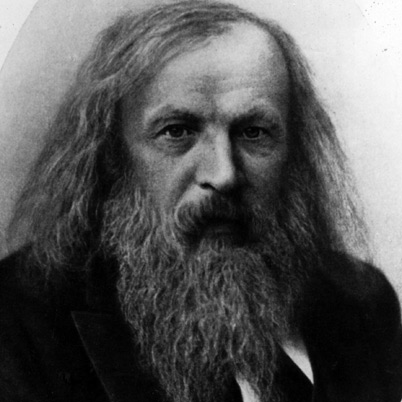
\includegraphics[height=4cm]{Images/mendeleev.jpg}};
	  	\pause
		\node (img2) at (img1.south) [yshift=-1cm] {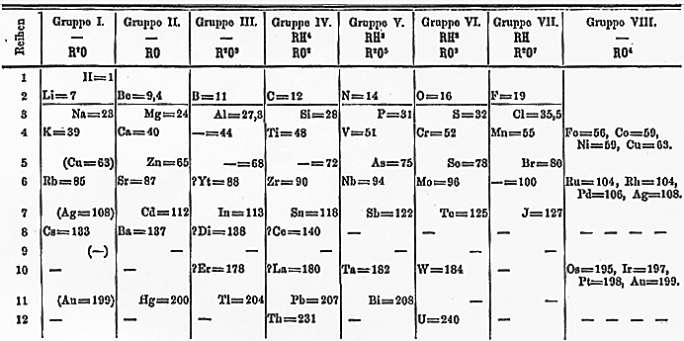
\includegraphics[width=\textwidth]{Images/periodic_table.png}};
	\end{tikzpicture}

	\end{column}
	\end{columns}
\end{frame}

\begin{frame}
	\frametitle{Example 2.}
	\framesubtitle{Orbits of Uranus and Mercury}

	\begin{columns}
	\begin{column}{0.5\textwidth}
		\includegraphics<1->[width=\textwidth]{Images/uranus.png}
		\begin{itemize}
			\item<1-> In 1841, it was noticed that Uranus' orbit was slightly off from predictions. 
			\item<2-> This observation led to the discovery of Neptune in 1846.
		\end{itemize}
	\end{column}
	\begin{column}{0.5\textwidth}
		\includegraphics<3->[width=\textwidth]{Images/mercury.jpg}
		\begin{itemize}
			\item<3-> In 1859, a similar problem emerged with the orbit of mercury
			\item<4-> This issue wasn't solved until Einstein's theory of general relativity superseded Newton's gravity in 1915.
		\end{itemize}


	\end{column}
	\end{columns}
\end{frame}




\begin{frameb}{w}{Images/gravitational-lens-1.jpg}
	\frametitle{Other evidence}
	\framesubtitle<2->{Gravitational Lensing}
\end{frameb}

\begin{frameb}{h}{Images/gravitational-lens-diagram.jpg}
	\frametitle{Gravitational Lensing}
\end{frameb}

\begin{frameb}{h}{Images/gravitational-lens.jpg}
	\frametitle{Gravitational Lensing}
\end{frameb}

\begin{frame}
	\frametitle{Other evidence}
	\framesubtitle{Structure formation}
\end{frame}

\plainframe{
	\movie[width=\textwidth,height=\textheight]{}{Movies/structure_formation.mp4}	
	}





\begin{frameb}{w}{Images/sdss.jpg}
	\frametitle{Other evidence}
	\framesubtitle{Structure formation}
\end{frameb}

\begin{frameb}{w}{Images/Planck-Map.jpg}
	\frametitle{Other evidence}
	\framesubtitle{Cosmic Microwave Background}
\end{frameb}

\begin{frame}
	\frametitle{What could dark matter be?}



	\begin{columns}
	\begin{column}{0.5\textwidth}
	\begin{description}
		\item<1->[MACHOs:] Massive Astrophysical Compact Halo Objects.
		\item<2->[WIMPs:] Weakly Interacting Massive Particles.
		
	\end{description}
	\end{column}
	\begin{column}{0.5\textwidth}
		\includegraphics<1->[width=\textwidth]{Images/Black_Hole.jpg}	

		\includegraphics<2->[width=\textwidth]{Images/dark_matter_halo.jpg}	
	\end{column}
	\end{columns}

\end{frame}
